\section{Limites et perspectives}

\subsection{}

\begin{frame}{Les limites de l'étude}
    Modèle mécanique simple
    \begin{itemize}
        \item Bras 2D
        \item Seulement 2 articulations
        \item Pas de redondance du bras dans l'espace de la tâche ($\ostate \rightarrow \jstate$)
    \end{itemize}
    ~\\
    Modèle de muscle simplifié
    \begin{itemize}
        \item Modèle linéaire
        \item Pas d'élasticité
        \item Modèle réactif
    \end{itemize}
    ~\\
    Coût énergétique des solutions trop élevé
\end{frame}

\begin{frame}{Perspectives}
    \begin{columns}
        \begin{column}{0.50\textwidth}
            Apprentissage du contrôle moteur
            \begin{itemize}
                \item Apprendre dans l'espace de la tâche
                \item Vaincre la \og{}malédiction de la dimensionalité\fg{}
                \item L'adaptation motrice et la réoptimisation
            \end{itemize}
        \end{column}
        \begin{column}{0.50\textwidth}
            \begin{center}
                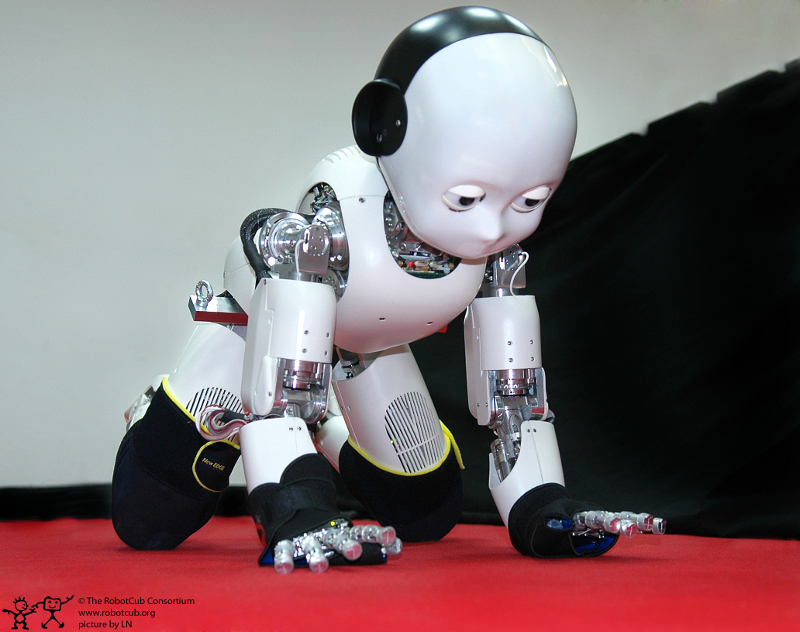
\includegraphics[width=.95\linewidth]{fig/icub3_light}
            \end{center}
        \end{column}
    \end{columns}
\end{frame}
